\documentclass[12pt,a4paper]{article}
\usepackage[width=.75\textwidth]{caption}
\usepackage{graphicx}
\usepackage{authblk}
\usepackage{amsmath}
\usepackage{amsfonts}
\usepackage{braket}
\usepackage{epigraph}
\usepackage{amssymb}
\usepackage{amsthm}
%\usepackage{mathrsfs}
\usepackage[mathscr]{euscript}
\usepackage[top=2cm, bottom=2cm, left=2cm, right=2cm]{geometry}
\usepackage{fancyhdr}

\theoremstyle{myrule}
\newtheorem{myrule}{Rule}[section]

\newtheorem{theorem}{Theorem}[section]
\newtheorem{corollary}{Corollary}[theorem]
\newtheorem{lemma}[theorem]{Lemma}

\setlength{\epigraphwidth}{0.8\textwidth}

\pagestyle{fancy}
\begin{document}

%title and author details
\title{Multi-Observer Quantum Mechanics from Classical Bayesian Inference}
\author[1]{Kevin Player\footnote{kjplaye@gmail.com}}

\maketitle


\epigraph{Solipsism may be logically consistent with present Quantum Mechanics, Monism in the sense of Materialism is not.}{Eugene Wigner}

\abstract{We present several quintessential quantum ideas and shed them in a classical light.  We argue how quantum information theory can be understood as a generalization of classical information theory in a nonstandard way (without density matrices).  In fact, we show how classical information theory can be embedded in quantum information theory using zero phase wavefunctions.  We employ this embedding to motivate a new multi-observer extension of quantum mechanics. Finally, we outline an experiment to test the existence of our multi-observer theory.}

\section{Some Thought Experiments}
Lets start with a 3-bit example, where each bit is realized by coins which are either heads (H) or tails (T).  With these 3 coins in hand, we conduct some thought experiments.  The ideas that we encounter all extend without loss of generality to any finite set and often to more general continuous densities.
\subsection{Classical Sequences}
Let us try to describe the situation once we throw the 3 coins.  Let
\[
x_i \in \{H,T\}
\]
be the outcome for the throws $i$ = $1,2,3$ and let $x = (x_1, x_2, x_3)$ denote the resulting sequence or tribit.  Let $C$ be the set of 8 possible tribits.  Nominally, we have 3 degrees of freedom to describe the tribit.  Lets move on and generalize using classical statistics.
  
\subsection{Classical Information Theory}
In the following subsections we outline an epistemic treatment of classical information where we try to represent our classical knowledge of the 3 coin ensemble.

\subsubsection{Rules for Constructing Knowledge Statements}
We want to describe a classical probabilistic knowledge statement\footnote{Whenever we say ``statement'' in this paper, we mean knowledge statement, or Bayesian belief statement.} about the coins.  We will construct our statements using some simple rules.
\begin{myrule}
\label{rule1}
For any tribit $x \in C$ we have the knowledge statement $b_x$, that says we know $x$ with certainty or probability 1.  We call this a basic statement.
\end{myrule}
There are 8 tribits, so there are 8 basic statements.
\begin{myrule}
 \label{rule2}
  A classical logical convex superposition can be made for any probabilistic statements $s_1$ and $s_2$ and $\alpha \in [0,1]$
  \begin{equation}
  \label{super}
  \text{super}_\alpha(s_1,s_2) = \alpha s_1 + (1 -\alpha) s_2.
  \end{equation}
This formal combination means to take statement $s_1$ with probability $\alpha$ and statement $s_2$ with probability $(1-\alpha)$; This is a new statement.
\end{myrule}

\subsubsection{Distributions on the Ensemble}

Next consider the set $P(C)$ of probability distributions on tribits.  We identify the 8 tribits $x$ with the integers $i=0,\cdots,7$, by using the binary expansion of $i$ and mapping $0 \mapsto H$ and $1 \mapsto T$ (for instance $5 \mapsto THT$).

For each $p$ in $P$ we let $p_i$ be the probability of the tribit $i$ (for instance $p_5$ is the probability of seeing $THT$.)  Then $p_i$ completely characterizes $p$ in the following way.  We can regard $p$ as living in an 8 dimensional space $\mathbb{R}^8$, which we call $X_3$ by taking
\[
p \mapsto (p_i) \in X_3.
\]
Let $\mathcal{O}(S)$ be the set of knowledge statements on $S$ built up from repeatedly applying the Rules \ref{rule1} and \ref{rule2}.
\begin{lemma}
  $\mathcal{O}(C)$ = $P(C)$
\end{lemma}
\begin{proof}
  Repeatedly applying superpositions starting with the basic statements and then also to the resulting sub-statements allows us to construct any probability distribution on tribits.  This can seen by inductively extending the distribution
  \[
  \eta_k = \gamma_k (p_0, \cdots, p_{k-1}, 0, \cdots)
  \]
  to
  \[
  \eta_{k+1} = \gamma_{k+1} (p_0, \cdots, p_{k}, 0, \cdots)
  \]
  using
  \[
  \eta_{k+1} = super_\alpha(\eta_k,b_k)
  \]
  for appropriate choices of normalizations $\gamma_k, \gamma_{k+1}$ and $\alpha$.
\end{proof}

A general knowledge statement $\eta \in P$ combines the basic statements $b_0, \cdots, b_7$ using coefficients $p_i$,
\[
  p_0,\cdots,p_{7} \in \mathbb{R}^+,
\]
so that $\eta = \sum p_i b_i$.  To be a statistical distribution we need it to be normalized with $\sum p_i = 1$.  Note that now (\ref{super}) is more than just a formal relation since it actually holds linearly inside of $X_3$.

We also  pause to note that each coin corresponds to a 2 dimensional space $X = \langle H, T \rangle$ spanned by formal vectors $H$ and $T$.  The 8 dimensional space $X ^ {\otimes 3}$ has a basis with vectors like $T \otimes H \otimes T$.  In this way, the space of classical knowledge statements of the ensemble, $X_3$, is naturally identified with the tensor power $X^{\otimes 3}$ by sending
\[
(x_1,x_2,x_3) \mapsto x_1 \otimes x_2 \otimes x_3.
\]
In general the classical knowledge statements about $n$ bit ensembles naturally live in $X ^ {\otimes n}$.
\begin{lemma}
  $\mathcal{O}(A \cup B) = \mathcal{O}(A) \otimes \mathcal{O}(B)$
\end{lemma}
\begin{proof}
  The proof is the same as above.  We find that $(a,b) \mapsto a \otimes b.$
\end{proof}

\subsubsection{Bayesian Projections as Classical Wave Function Collapse}
\label{proj}
We don't always get to measure the exact tribit.  For instance, we might only get to know that the first coin is $T$ and that the 2nd and 3rd coins are the same.  This corresponds to an subset of $\{0,\cdots,7\}$, which we will call
\[
\begin{split}
  S &= \{s \in \{0,\cdots,7\} | c_1(s) = T, c_2(s) = c_3(s) \} \\
    & = \{4,7\} \hspace{0.4 in} \text{(THH, TTT)}
\end{split}
\]
where $c_i(s)$ is the value $x_i$.  We will use $S$ as an example in the remaining text.

\begin{figure}[h]
\centering
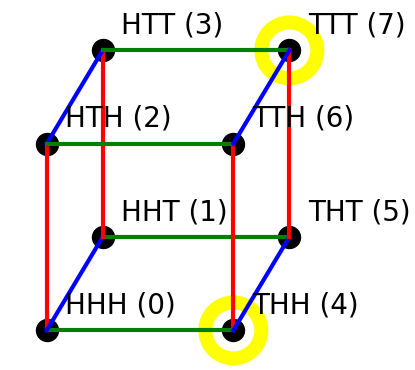
\includegraphics[scale=0.6]{cube.png}
\caption{Coin sequences with $S$ circled in yellow.}
\label{masslessshell}
\end{figure}

Someone could make a measurement that tells them that the state is in $S$ and nothing else.  This would be a specific case of a projection measurement.  The statement becomes zero exactly on $p_i$ where $i \not \in S$ and just renormalizes $p_i$ on the remaining $i \in S$.  It is exactly
\begin{equation}
\label{sdist}
(p_0,\cdots,p_7) = \left(0,0,0,0,\frac{1}{2},0,0,\frac{1}{2}\right)
\end{equation}
\subsubsection{Bayesian Inference as General Classical Wave Function Collapse}
A more general type of measurement is a probabilistic measurement.  Someone could learn that there is a 95\% chance that the state is in $S$.  In full generality we will call such a probabilistic observation $\mathcal{O}$.  We can figure out how to update our knowledge statement from $p_i$, to $\hat{p_i}$, using a relative\footnote{In the ratio, the contribution of $P(\mathcal{O})$ is canceled out and accounted for during normalization.  $P(\mathcal{O})$ only holds significance prior to its observation and it doesn't require consideration during the update process.} version of Bayes's rule
\[
  \frac{\hat{p_i}}{\hat{p_j}} = \underbrace{\frac{P(i | \mathcal{O})}{P(j | \mathcal{O})}}_\text{Posterior}
                              = \underbrace{\frac{P(\mathcal{O} | i)}{P(\mathcal{O}|j)}}_\text{Bayes Factor}  \hspace{0.07 in}  \underbrace{\frac{p_i}{p_j}}_\text{Prior}
\]
Pulling out the Bayes factor we find that we just multiply by the likelihood and re-normalize
\[
  \hat{p_k} =  P(\mathcal{O} | k) \hspace{0.07 in} p_k.
\]
A special case are projections $P(\mathcal{O} | k) \in \{0,v\}$, for some fixed value $v$, like the $S$ projection case in section \ref{proj}.  We call these Bayesian projections.

\subsubsection{Classical Correlation as Classical Entanglement}
Finally, we can also consider again the distribution (\ref{sdist}). We know the first coin is T, which we promptly throw away.

We have $HH$ or $TT$ with equal probabilities for the second and third coins.  If we give the second coin to Alice and the third coin to Bob then we have a classical correlation.  If Bob finds that the third coin is $T$ then we know that Alice will also find that the second coin is $T$ (and similarly for $F$).  The reduction is purely epistemic, it is the separate knowledge of Alice and Bob that is changing.  Classical correlation should be very familiar from every day experience.

\subsection{Quantum Information Theory}
\subsubsection{Classical to Quantum Embedding}
General quantum information\footnote{We are purposely leaving out density matrices and POVMs and just dealing with pure states.} about 8-qubits can be expressed as a wave function.
\[
   q_0,\cdots,q_{7} \in \mathbb{C}
\]
with $\sum |q_i|^2 = 1$.  The Born rule is ostensibly a map $q_i \mapsto |q_i|^2 = p_i$ to classical probability.  Here we can instrument all of the classical information theoretic constructs by restricting the phase\footnote{We consider negative values as 180 degrees out of phase, so zero phase means non-negative real.} of $q_i$ to be zero.  We can map backward $p_i \mapsto \sqrt{p_i} = q_i$; which commutes with the Born rule (subject to normalization):

{
\renewcommand{\arraystretch}{0.1}
\[
\text{(Quantum)} \hspace{0.3 in}
\mathbb{C}^n \begin{array}{c} \twoheadrightarrow \\ \hookleftarrow \end{array}
(\mathbb{R}_{\ge 0})^n
\hspace{0.3 in} \text{(Classical)} 
\]
}

So quantum information theory needs to generalize the classical.  In particular, quantum measurement and entanglement restrict to classical measurement and classical correlation for zero phase.

\subsubsection{Bayesian Projection}
We illustrate zero phase Bayesian projection with an example.

Within the embedding we define a projection operator $\pi$ which projects onto the space generated by the subset $S$, from the previous subsection
\[
\pi = \sum_{i \in S} \ket{i} \bra{i}.
\]
Then let $A$ be any operator with an eigenspace, with eigenvalue $\lambda$, equal to the image of $\pi$.  An observation of $\lambda$ would correspond to an application of $\pi$, which is a Bayesian projection in the classical picture.

\subsubsection{Bayesian Inference}
Consider, in the fashion of \cite{nielsenchuang}, a more general measurement with matrix $M_\mathcal{O}$ which is diagonal with entries
\[
   M_\mathcal{O}(i,i) = \sqrt{P(\mathcal{O} | i)}
\]
This implements classical Bayesian inference using zero phase wavefunctions.


\subsubsection{Entropy}
Von Neumann entropy is left out of this note since it is not a generalization of classical entropy in the manner presented here.  This is because the zero phase classical wavefunctions are pure states which all have zero Von Neumann entropy.

\section{Overview of the Generalization}

The quantum mechanical concepts wave function collapse, entanglements and ensembles are direct generalizations of the classical information theoretic concepts of Bayesian inference, correlation and statistical ensembles respectively.  This is not to say that they are not strange, but to say that they need to be generalizations of the classical concepts.  Wave function collapsing should generalize Bayesian inference and classical measurement.  Entanglement should be a generalization of classical correlation.  This is enough to motivate new ways of doing quantum mechanics, which we will encounter in the next sections.

\subsection{Multi-Observer Quantum Mechanics}
We focus on quantum wave function collapse as a generalization of classical Bayesian inference.  We can implement the classical Bayesian inference within zero phase quantum mechanics as outlined above.  So the classical Bayesian theory has a direct tie in; that observation and measurement occur in tandem with a change in knowledge\footnote{This change in knowledge is tangible, it always occurs as a transfer of matter/energy from the environment to the observer \cite{thrust}.}.  

In the classical theory, knowledge is local to the observer\footnote{Note that current quantum theory is a theory of one observer, usually the experimenter in a lab.  An immediate subject is quantum key distribution(QKD), which requires at least three observers, Alice, Bob, and Eve; the security of QKD depends on multi-observer quantum ontology.}, multiple observers each have their own knowledge.  For instance, Wigner's friend and Wigner each have their own classical knowledge.  It would seem then that Wigner's friend and Wigner must have different zero phase wavefunctions as well, if they are to be generalizing classical knowledge.  This is our prediction for multi-observer quantum physics, that every observer has a local wavefunction. 

\subsection{Prediction and Experiment}

We predict that multi-observer quantum mechanics will be required for a proper generalization of classical knowledge.  We propose an experiment where we inject an ``observer'' into a quantum eraser\footnote{Here we probe the boundaries of what constitutes an observer and a measurement.  We claim that all versions of observer and measurement will be detectable in this experiment whenever it can be done.}.  The injected observer will have to be a small apparatus that is
\begin{itemize}
   \item able to record a measurement $\psi$ of the eraser particle path.
   \item able to forget the measurement $\psi$.
   \item able to demonstrate that a measurement was made with a record $\rho$.
\end{itemize}
Let $\phi$ be the lab technician's wavefunction.  In $\phi$ the apparatus is entangled with the subject particles in the eraser experiment.  We need to find out if there is another wavefunction in play that is not just part of $\phi$.  The key here is that the apparatus is able to demonstrate that it ``knew'' something, or in other words that another wavefunction $\psi$ existed, using $\rho$.

The apparatus can not keep $\psi$ for proper erasure, but must ``forget'' it.  Observed erasure, via an interference pattern, proves that $\psi$ is not a part of $\phi$.  Finally, there should be a record $\rho$ in the apparatus that it did at one point in time record a measurement $\psi$.  Receipt of the report $\rho$ and eraser interference pattern together show that $\psi$ and $\phi$ were necessarily part of a two-observer system.

\section{Acknowledgments}
Thanks to Erik Ferragut and Dan Justice for useful discussions.

\bibliographystyle{ieeetr}
\bibliography{bibliography}

\end{document}
